\section*{Question 1}

\subsection*{a.}

\begin{flalign*}
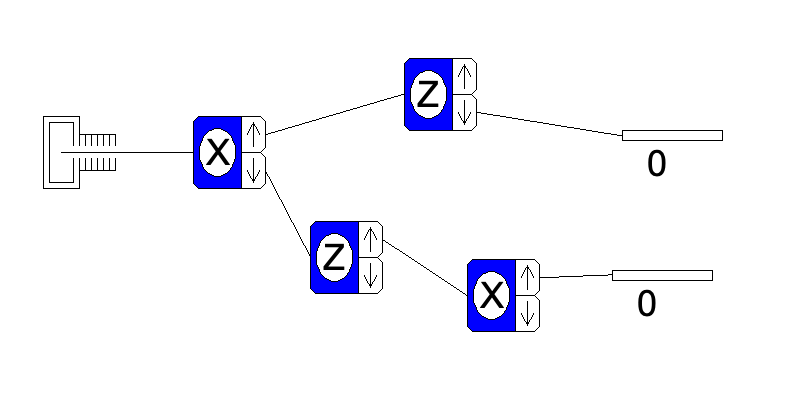
\includegraphics[scale=0.4]{images/1a.png}
\end{flalign*}

\subsection*{b.}

\begin{flalign*}
\phantom{aaaa}
    P_{-z} &= \left| \braket{-z \; | +x} \right|^2 && \\
           &= \left| \bra{-z} \left( \frac{1}{\sqrt{2}}\ket{+z} + \frac{1}{\sqrt{2}}\ket{-z} \right) \right|^2 && \\
           &= \left| \frac{1}{\sqrt{2}}\braket{-z \; | +z} + \frac{1}{\sqrt{2}}\braket{-z \; | -z} \right|^2 && \\
           &= \frac{1}{2} && \\
\end{flalign*}

\begin{flalign*}
\phantom{aaaa}
    P_{+x} &= \left| \braket{+x \; | +z} \right|^2 \; \left| \braket{+z \; | -x} \right|^2 && \\
           &= \left| \left(\frac{1}{\sqrt{2}}\bra{+z} + \frac{1}{\sqrt{2}}\bra{-z}\right) \ket{+z} \right|^2 \; \left| \bra{+z}\left(\frac{1}{\sqrt{2}}\ket{+z} - \frac{1}{\sqrt{2}}\ket{+z}\right)  \right|^2 && \\
           &= \left| \frac{1}{\sqrt{2}}\braket{+z \; | +z} + \frac{1}{\sqrt{2}}\braket{-z \; | +z} \right|^2 \; \left| \frac{1}{\sqrt{2}}\braket{+z \; | +z} - \frac{1}{\sqrt{2}}\braket{+z \; | -z} \right|^2 && \\
           & && \\
           &= \left(\frac{1}{2}\right) \left(\frac{1}{2}\right) && \\
           & && \\
           &= \frac{1}{4} && \\
\end{flalign*}

\subsection*{c.}

Atoms expected at $-z$ port:

\begin{flalign*}
\phantom{aaaa}
    & 10000 \cdot \frac{1}{2} \cdot \frac{1}{2} = 2500 && \\
\end{flalign*}

\noindent
Atoms expected at $+x$ port:

\begin{flalign*}
\phantom{aaaa}
    & 10000 \cdot \frac{1}{2} \cdot \frac{1}{4} = 1250 && \\
\end{flalign*}

\subsection*{d.}

\begin{flalign*}
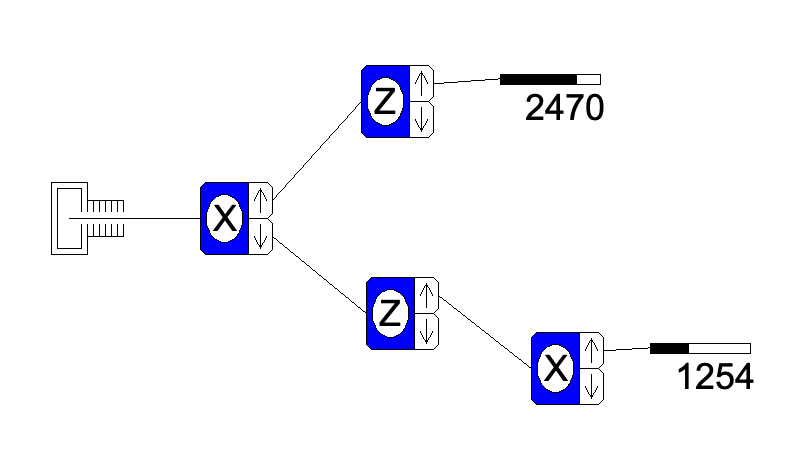
\includegraphics[scale=0.4]{images/1d.png}
\end{flalign*}

\noindent
The simulated results are consistent with the theoretical results (within a reasonable margin of error). \\

\noindent
Using a larger number of atoms in the simulation would result in convergence to the theoretical results.


\section*{Question 2}

\subsection*{a.}

\begin{flalign*}
\begin{tabular}{ c | c | c | c | c }
    Iteration & $+x$ & $-x$ & $+z$ & $-z$ \\
    \hline
    &  & & \\
    1  & 2485 & 0 & 1254 & 1222 \\
    &  & & \\
    2  & 2518 & 0 & 1248 & 1274 \\
    &  & & \\
    3  & 2493 & 0 & 1260 & 1227 \\
    &  & & \\
    4  & 2431 & 0 & 1280 & 1206 \\
    &  & & \\
    5  & 2514 & 0 & 1174 & 1290 \\
    &  & & \\
    6  & 2453 & 0 & 1250 & 1268 \\
    &  & & \\
    7  & 2515 & 0 & 1261 & 1307 \\
    &  & & \\
    8  & 2516 & 0 & 1262 & 1276 \\
    &  & & \\
    9  & 2514 & 0 & 1269 & 1246 \\
    &  & & \\
    10 & 2427 & 0 & 1251 & 1246 \\
\end{tabular}
\end{flalign*}


\subsection*{b.}

\noindent
From the simulations, the average value for the number of atoms with spin $+x$ is given by:

\begin{flalign*}
\phantom{aaaa}
    & \frac{1}{10} \sum_{i=1}^{10} +x_i = 2486.6 && \\
\end{flalign*}

\newpage

\noindent
The theoretical probability is found like so:

\begin{flalign*}
\phantom{aaaa}
    P_{+x} &= \left| \braket{+x \; | +x} \right|^2 \; \left| \braket{+x \; | +z} \right|^2 && \\
           &= \left| \braket{+x \; | +z} \right|^2 && \\
           &= \left| \left(\frac{1}{\sqrt{2}}\bra{+z} + \frac{1}{\sqrt{2}}\bra{-z}\right)\ket{+z} \right|^2 && \\
           &= \left| \frac{1}{\sqrt{2}}\braket{+z \; | +z} + \frac{1}{\sqrt{2}}\braket{-z \; | +z} \right|^2 && \\
           &= \frac{1}{2} &&
\end{flalign*}


\subsection*{c.}

\noindent
From the simulations, the average value for the number of atoms with spin $+z$ is given by:

\begin{flalign*}
\phantom{aaaa}
    & \frac{1}{10} \sum_{i=1}^{10} +z_i = 1250.9 && \\
\end{flalign*}

\noindent
The theoretical probability is found like so:

\begin{flalign*}
\phantom{aaaa}
    P_{+x} &= \left| \braket{-z \; | -x} \right|^2 \; \left| \braket{-x \; | +z} \right|^2 && \\
           &= \left| \bra{-z}\left( \frac{1}{\sqrt{2}}\ket{+z} - \frac{1}{\sqrt{2}}\ket{-z} \right) \right|^2 \; \left| \left( \frac{1}{\sqrt{2}}\bra{+z} - \frac{1}{\sqrt{2}}\bra{-z} \right)\ket{+z} \right|^2 && \\
           &= \left| \frac{1}{\sqrt{2}}\braket{-z \; | +z} - \frac{1}{\sqrt{2}}\braket{-z \; | -z} \right|^2 \; \left| \frac{1}{\sqrt{2}}\braket{+z \; | +z} - \frac{1}{\sqrt{2}}\braket{-z \; | +z} \right|^2 && \\
           &= \left(\frac{1}{2}\right) \left(\frac{1}{2}\right) && \\
           &= \frac{1}{4} &&
\end{flalign*}

\subsection*{d.}

\noindent
The X analyzer immediately before the second X analyzer prepares the atoms in the $+x$ state. As such,
the probability of atoms being detected at the $-x$ port is 0.

\section*{Question 3}

\subsection*{a.}

\noindent
The quantom state $\ket{\psi}$ must be normalized so that their probabilities |$\braket{\pm z \; | \psi}$|
sum to 1. \\

\noindent
If all quantum states are not normalized, the total probability of all quantum states will not sum to 1,
violating basic probability theory.

\subsection*{b.}

\noindent
Due to the law of large numbers, the experimental uncertainty (error) will converge to
the theoretical value as the expirement is repeated a large number of times.

\noindent
However, the theoretical uncertainty (due to the uncertainty principle) will
not change as the experiment is repeated.

\subsection*{c.}

\noindent
If the SG-analyzers are not perfectly aligned, error will be introduced into the experiment (obviously).
Specifically, an analyzer which is mis-aligned in the $+z$ direction (for example) will introduce
bias (error) into the $+z$ and $-z$ measurements.